\chapter{Despliegue del modelo}\label{chp-03}
\epigraph{Less is more.}{Ludwig Mies van der Rohe}

\section{Problemática y solución}

Nos encontramos en esta situación: el modelo ha sido entrenado o está siendo desarrollado por otro equipo.
Nuestro trabajo consiste en implementarlo en un entorno de producción para que pueda ser utilizado por los usuarios finales.

Este problema puede ser abordado de varias formas, y la solución estará altamente condicionada por los requisitos del proyecto.
Al no tener ningún requisito impuesto para este trabajo, surgen muchos interrogantes cuya respuesta no es trivial:

\begin{itemize}
    \item \textbf{Aspecto final de la solución}: ¿Cómo se va a utilizar el modelo? ¿Qué tipo de interfaz se va a utilizar? ¿Qué tipo de dispositivo se va a utilizar?
    \item \textbf{Requisitos de la solución}: ¿Qué requisitos de rendimiento tiene la solución? ¿Con qué riesgos podemos encontrarnos? ¿Qué requisitos de escalabilidad tiene la solución?
    \item \textbf{Arquitectura de la solución}: ¿En qué lenguaje se va a implementar la solución? ¿Qué tipo de arquitectura se va a utilizar? ¿Qué tipo de servidores se van a utilizar?
    
\end{itemize}

En este caso, se ha optado por simplificar el aspecto final de la solución para centrarnos en el despliegue del modelo.
Se ha decidido crear una interfaz web que permita a los usuarios finales interactuar con el modelo, y una implementación mediante contenedores Docker para facilitar el despliegue en cualquier entorno.

\section{Enfoque escogido}
En un principio se pensó en realizar inferencia en tiempo real, es decir, que la aplicación, una vez iniciada, estuviera grabando continuamente y realizando predicciones.
Esta opción sin embargo, no ha podido ser llevada a cabo de forma exitosa debido al tiempo de respuesta que ofrece el servidor en el que se ha desplegado la aplicación.

Además, para implementarla de forma correcta, habría que añadir diversos mecanismos que ayuden a filtrar los audios y nos permitieran extraer muestras que pudieran ser utilizadas para realizar predicciones.
Esto implicaría detección de inicio y fin de actividad vocal, filtrado de silencios, etc.
La complicación de este proceso, unido al tiempo de respuesta del servidor, ha hecho que se descarte esta opción.

Finalmente, contamos con una aplicación web que permite a los usuarios finales grabar audios y obtener una predicción de la clase a la que pertenece el audio, se presuponen audios válidos para clasificar por emociones.
La aplicación está pensada para ser utilizada en una sola dirección: el usuario debe iniciar la grabación, grabar un mensaje, parar la grabación y esperar el resultado.
Una vez obtenido el resultado, puede volver a grabar otro mensaje.

La aplicación es accesible desde cualquier dispositivo que tenga un navegador web a través de la dirección \url{https://www.classifier-web.com/}.

\begin{figure}[htpb]
    \centering
    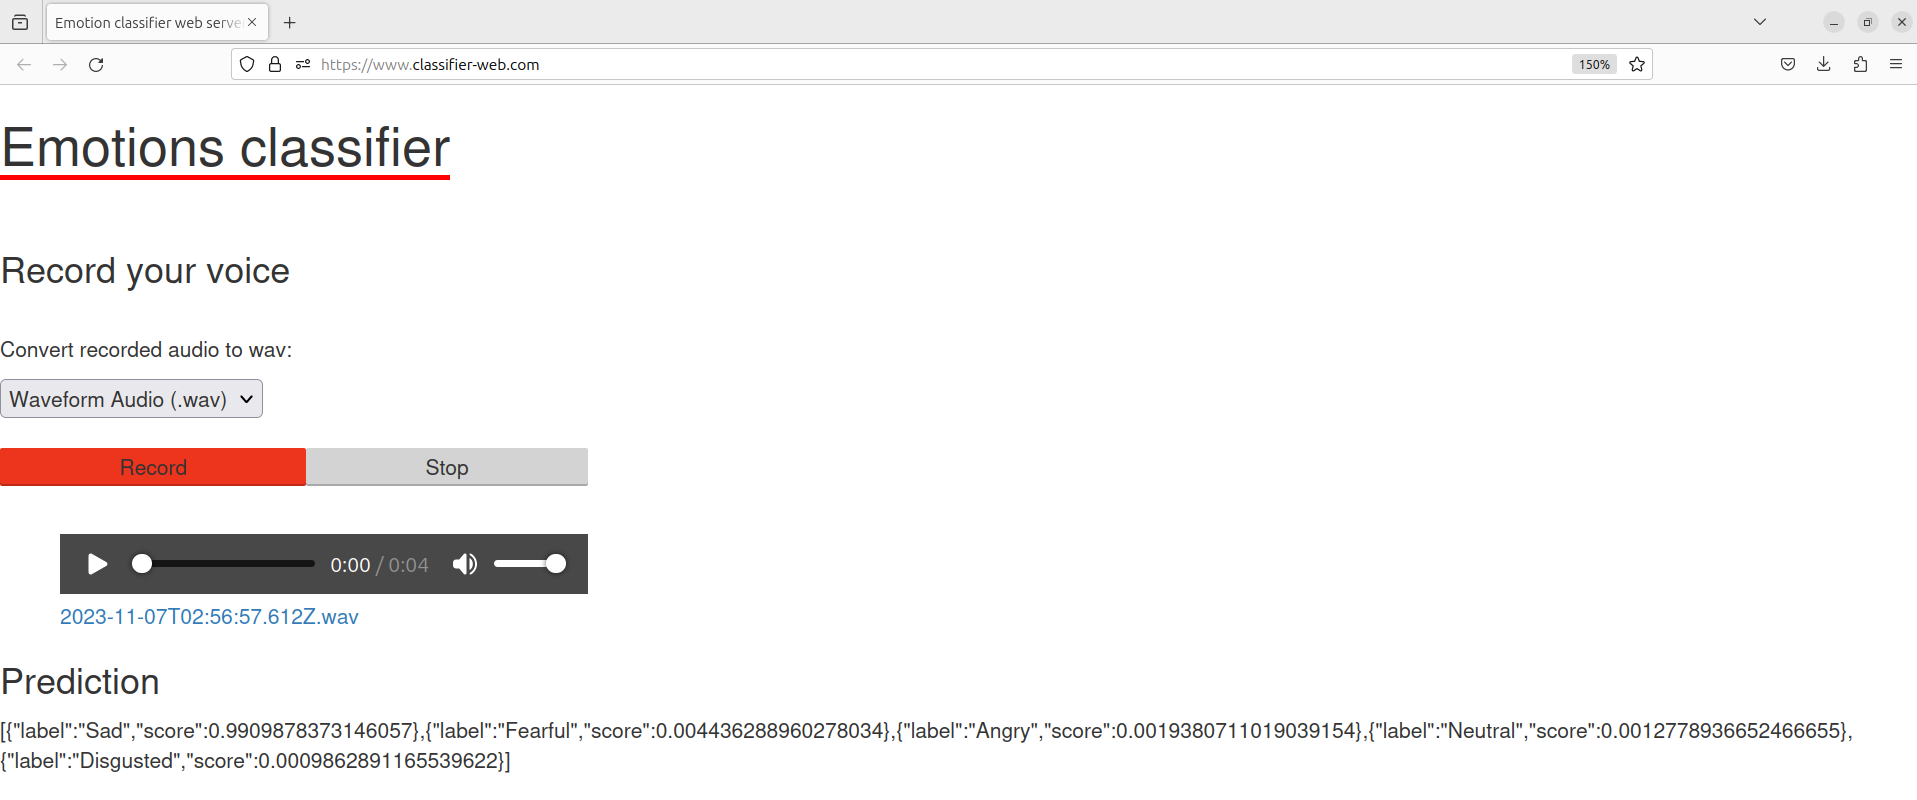
\includegraphics[width=0.8\textwidth]{cap3/images/interfaz-web.png}
    \caption{Resultado mostrado en la interfaz tras realizar una predicción}
    \label{fig:interfaz-web}
\end{figure}


\section{Aplicación web}
Una forma sencilla de crear una interfaz que sea accesible desde cualquier dispositivo es crear una aplicación web.

Aunque el modelo creado puede ser integrado utilizando cualquier lenguaje de programación, se ha optado por utilizar \textit{Python} para la implementación de la aplicación web.
\textit{Python} cuenta con una gran cantidad de librerías que facilitan la implementación de aplicaciones web, como \textit{Flask} o \textit{Django}, quizás las más populares.

Se ha optado por utilizar \textit{Flask}, debido a que es una librería más ligera que Django y a que es más sencilla de utilizar.
Además, contamos con cierta experiencia previa en el uso de \textit{Flask}, lo que nos permite acelerar el desarrollo de la aplicación.


\subsection{\textit{Flask}}
\textit{Flask} es un microframework para \textit{Python} que permite crear aplicaciones web de forma sencilla.

Está diseñado para ser extensible, por lo que es posible añadirle funcionalidades mediante extensiones, aunque en este caso no vamos a utilizar ninguna.
Sin embargo, estas extensinoes de alto nivel nos abren las puertas a posibles líneas futuras, como lecturas de bases de datos, autenticación de usuarios, etc.

Utilizar \textit{Python} para la creación web no siempre es la solución idónea, ya que existen otros lenguajes de programación que están más orientados a la creación de aplicaciones web.
Sin embargo, si no se tiene experiencia previa en estos lenguajes, o el objetivo es lanzar una aplicación web de forma rápida, \textit{Flask} es idóneo.
No estamos exentos de tener que crear plantillas en otros lenguajes propios de la web, como HTML, CSS o JavaScript, pero \textit{Flask} nos permite crear una aplicación web funcional en muy poco tiempo.


\subsection{Estructura de la aplicación}
Aunque \textit{Flask} ofrece muhas posibilidades, en este caso se ha optado por crear una aplicación web muy sencilla, que consta de dos partes principales.

Primero el modelo es cargado en memoria, y se crea una instancia de \textit{Flask}.
El modelo es cargado en memoria para evitar tener que cargarlo cada vez que se realiza una predicción, lo que se traduciría en un aumento del tiempo de respuesta de la aplicación.
Esto puede ralentizar sin embargo el arranque de la aplicaión, pero es una operación que se realiza una única vez.

Posteriormente se crean las rutas de la aplicación, que son las direcciones a las que se puede acceder desde un navegador web.
Contamos con la ruta principal, que es la que se utiliza para cargar la página principal de la aplicación, y la ruta de predicción, que es la que se utiliza para realizar las predicciones.

La ruta principal simplemente carga un fichero HTML que contiene el código de la página principal.

La ruta de predicción es llamada internamente mediante una petición POST lanzada por el código del lado del cliente escrita en \textit{JavaScript} cuando un usuario termina una grabación.
La grabación se guarda localmente en el servidor momentáneamente para que el modelo pueda realizar la predicción sobre ella, y posteriormente se borra, por cuestiones de espacio y privacidad.


\begin{lstlisting}[language=Python, caption={Aplicación Flask.}, label={lst:flask-app}]
from flask import Flask, request, jsonify, render_template, redirect
import os
import random

from transformers import pipeline

app = Flask(__name__)
pipe = pipeline("audio-classification", model="antonjaragon/emotions_6_classes_small")

@app.route("/", methods=["GET", "POST"])
def index():
predict = ""
if request.method == "POST":
    print("FORM DATA RECEIVED")

    if "file" not in request.files:
        return redirect(request.url)

    file = request.files["file"]
    if file.filename == "":
        return redirect(request.url)

    if file:
        
        predict = pipe(file.filename)



return render_template('index.html')

@app.route('/save_recording', methods=['POST'])
def upload():
if request.method == 'POST':
    f = request.files['audio_data']
    # audio folder is static/audios/random int/filename
    audio_folder = 'static/audios/' + str(random.randint(1, 100000000000000000))
    # create folder if not exists audio_folder
    if not os.path.exists(audio_folder):
        os.makedirs(audio_folder)
    f.save(os.path.join(audio_folder, f.filename))
    output = pipe(audio_folder + '/' + f.filename)
    # print(output)

    # delete the audio folder after prediction
    os.remove(audio_folder + '/' + f.filename)
    os.rmdir(audio_folder)

    return output


@app.route('/cache-me')
def cache():
return "server will cache this response"

@app.route('/info')
def info():

resp = {
    'connecting_ip': request.headers['X-Real-IP'],
    'proxy_ip': request.headers['X-Forwarded-For'],
    'host': request.headers['Host'],
    'user-agent': request.headers['User-Agent']
}

return jsonify(resp)

@app.route('/flask-health-check')
def flask_health_check():
return "success"
\end{lstlisting}


\subsection{Interfaz web}
El desarrollo de interfaces web es un mundo complejo, y no es el objetivo de este trabajo crear una interfaz especialmente atractiva, sino más bien que nos proporcione la funcionalidad básica.
Existen desarrolladores especializados únicamente en el desarrollo de interfaces web, y es un campo que requiere de un conocimiento muy amplio, además de experiencia.

Debido a tratar esta parte como algo secundario, sumado a la falta de conocimiento acerca del manejo de audios en la web, se ha optado por basar la interfaz en trabajo previo realizado por otros desarrolladores.
En concreto, se ha utilizado como base el proyecto con licencia para uso público alojado en \textit{GitHub} titulado \textit{Voice-to-text-with-Python-in-Flask} \cite{voice-to-text-with-python-in-flask}.

La interfaz web final es muy sencilla, y se puede ver en la \autoref{fig:interfaz-web}.
Contiene lo básico para que un usuario pueda realizar la grabación de un audio y obtener una predicción de la clase a la que pertenece el audio.



\section{Aplicación \textit{Flask} en producción}
\textit{Flask} integra un servidor web apto para entornos de desarrollo, que es el que se utiliza por defecto cuando se lanza la aplicación, llamado \textit{Werkzeug}.
Este servidor es muy sencillo de utilizar, pero no está pensado para ser utilizado en producción, ya que no está optimizado para soportar un gran número de peticiones simultáneas.


\subsection{\textit{Gunicorn}}
Para lanzar la aplicación en producción, se ha optado por utilizar \textit{Gunicorn}, un servidor web \textit{HTTP WSGI} (Web Server Gateway Interface)
para \textit{Python}.
Es uno de los servidores más utilizados para lanzar aplicaciones \textit{Flask} en producción, y es además recomendado en la documentación oficial de \textit{Flask}.

\textit{Gunicorn} es un servidor web que se encarga de gestionar las peticiones HTTP que llegan a la aplicación, y de lanzar procesos de la aplicación para atender estas peticiones.
Esto permite que la aplicación pueda atender varias peticiones simultáneamente, lo que se traduce en un aumento del rendimiento de la aplicación.

\begin{lstlisting}[language=bash, caption={Código guardado en 'wsgi.py'.}, label={lst:wsgi}]
from app import app
import os

if __name__ == "__main__":
    app.run(host='0.0.0.0', port=8000, debug=True)
    

\end{lstlisting}

\begin{lstlisting}[language=bash, caption={Comando para lanzar la aplicación con \textit{Gunicorn}.}, label={lst:gunicorn}]
    gunicorn -b 0.0.0.0:8000 wsgi:app
\end{lstlisting}

El \autoref{lst:gunicorn}, lanzará un servidor web en el puerto 8000, el puerto que se suele usar por defecto, que permite conexiones desde cualquier dirección IP.

El siguiente paso es configurar un servidor web que actúe como proxy inverso, para que las peticiones HTTP que lleguen al servidor web sean redirigidas al servidor \textit{Gunicorn}.


\subsection{\textit{Traefik}}
Para configurar el servidor web que actúe como proxy inverso, se ha optado por utilizar \textit{Traefik}.
Aunque \textit{Nginx} es quizás el servidor web más utilizado para realizar esta tarea, la elección de \textit{Traefik} se debe principalmente a su facilidad de configuración.

En la actualidad, \textit{Nginx} ofrece más funcionalidades, pero para este caso con una configuración básica es suficiente.
La mayor ventaja que nos ha brindado \textit{Traefik} es la facilidad de generar certificados SSL para la aplicación, lo que nos permite utilizar HTTPS.
Esto es importante, ya que si no se utiliza HTTPS, los navegadores web no permiten acceder al micrófono del dispositivo, lo que hace imposible la grabación de audios.

\begin{figure}[htpb]
    \centering
    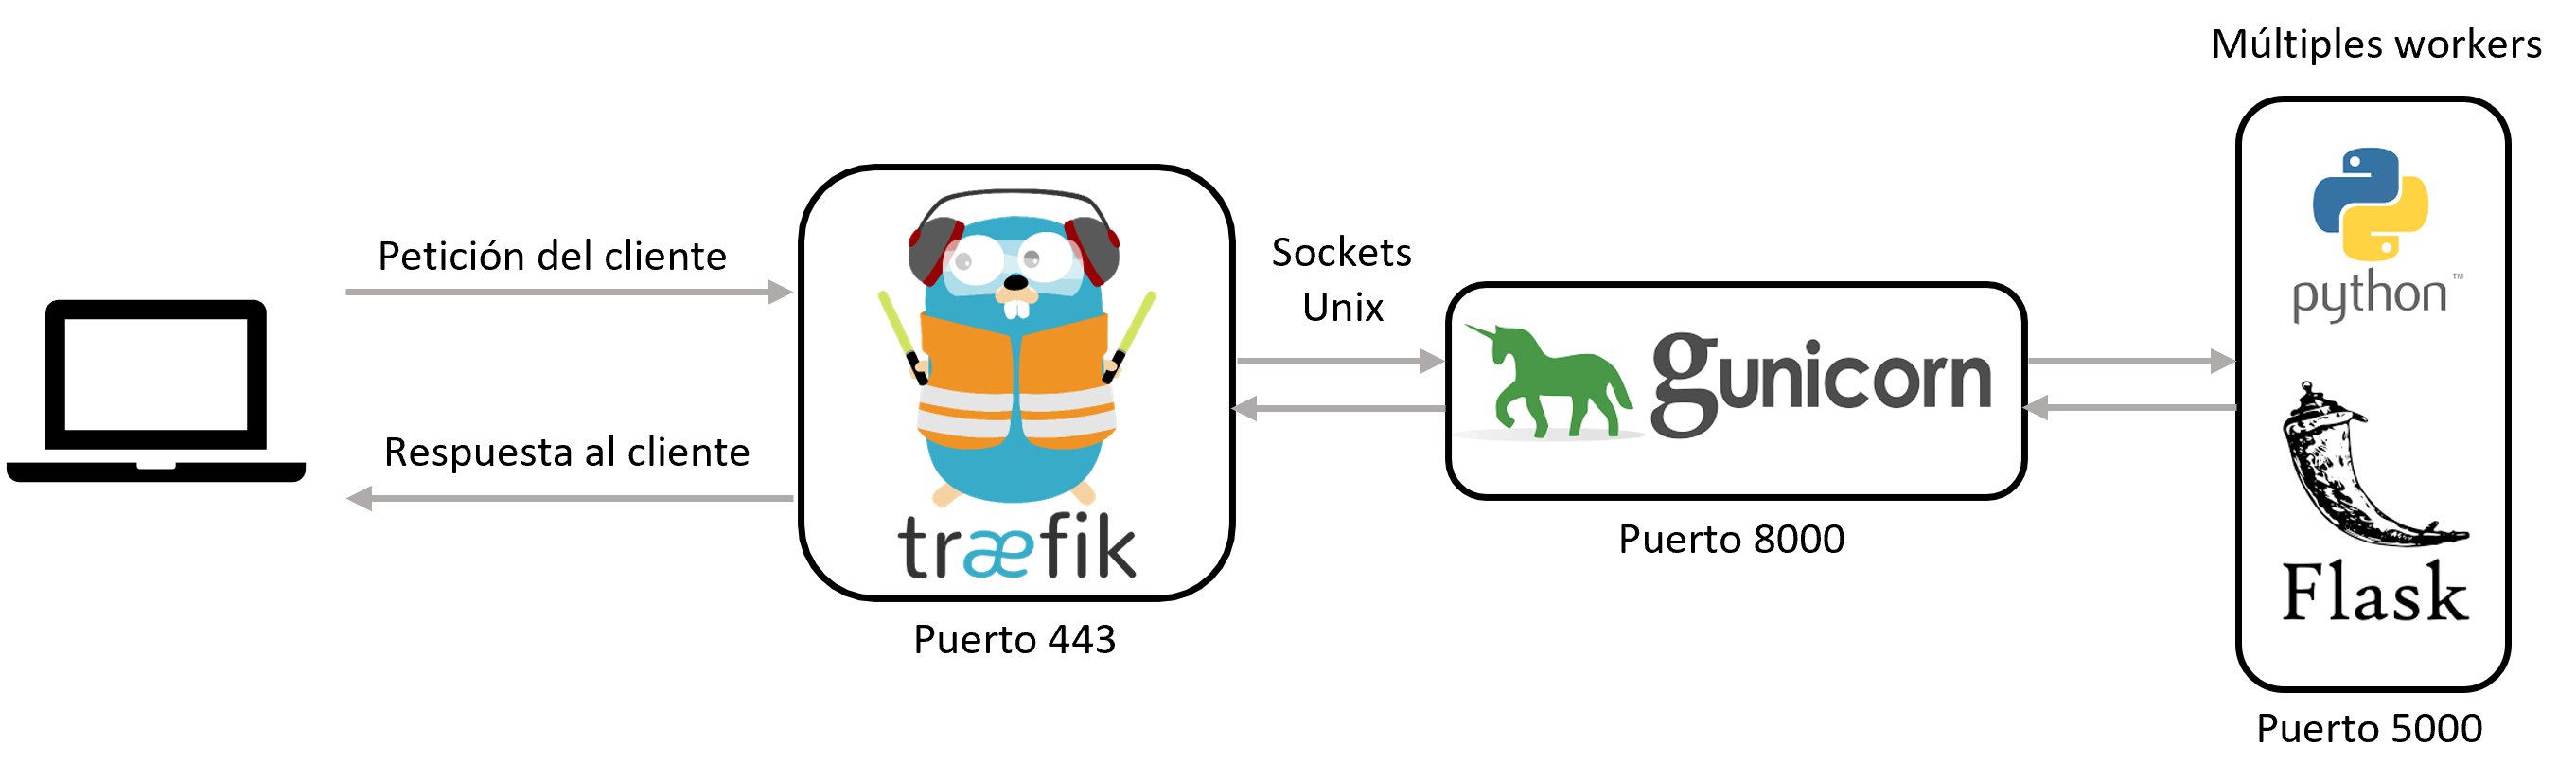
\includegraphics[width=0.8\textwidth]{cap3/images/arquitectura.png}
    \caption{Esquema completo del sistema}
    \label{fig:traefik}
    
\end{figure}



No es una tarea difícil de realizar correctamente para un desarrollador experimentado mediante un servidor web como \textit{Nginx}, pero es mucho más sencillo de realizar con \textit{Traefik}, y además, al contar con poca experiencia en este campo, nos ha permitido solventar este problema de forma rápida y sencilla.
Además, \textit{Traefik} aún está dando sus primeros pasos, y está ganando popularidad entre desarrolladores, por lo que quizás en un futuro sea una alternativa a \textit{Nginx} también en entornos reales de producción.

% """ insertar foto de \url{https://monitor.classifier-web.com} indicando admin:admin"""
\begin{figure}[htpb]
    \centering
    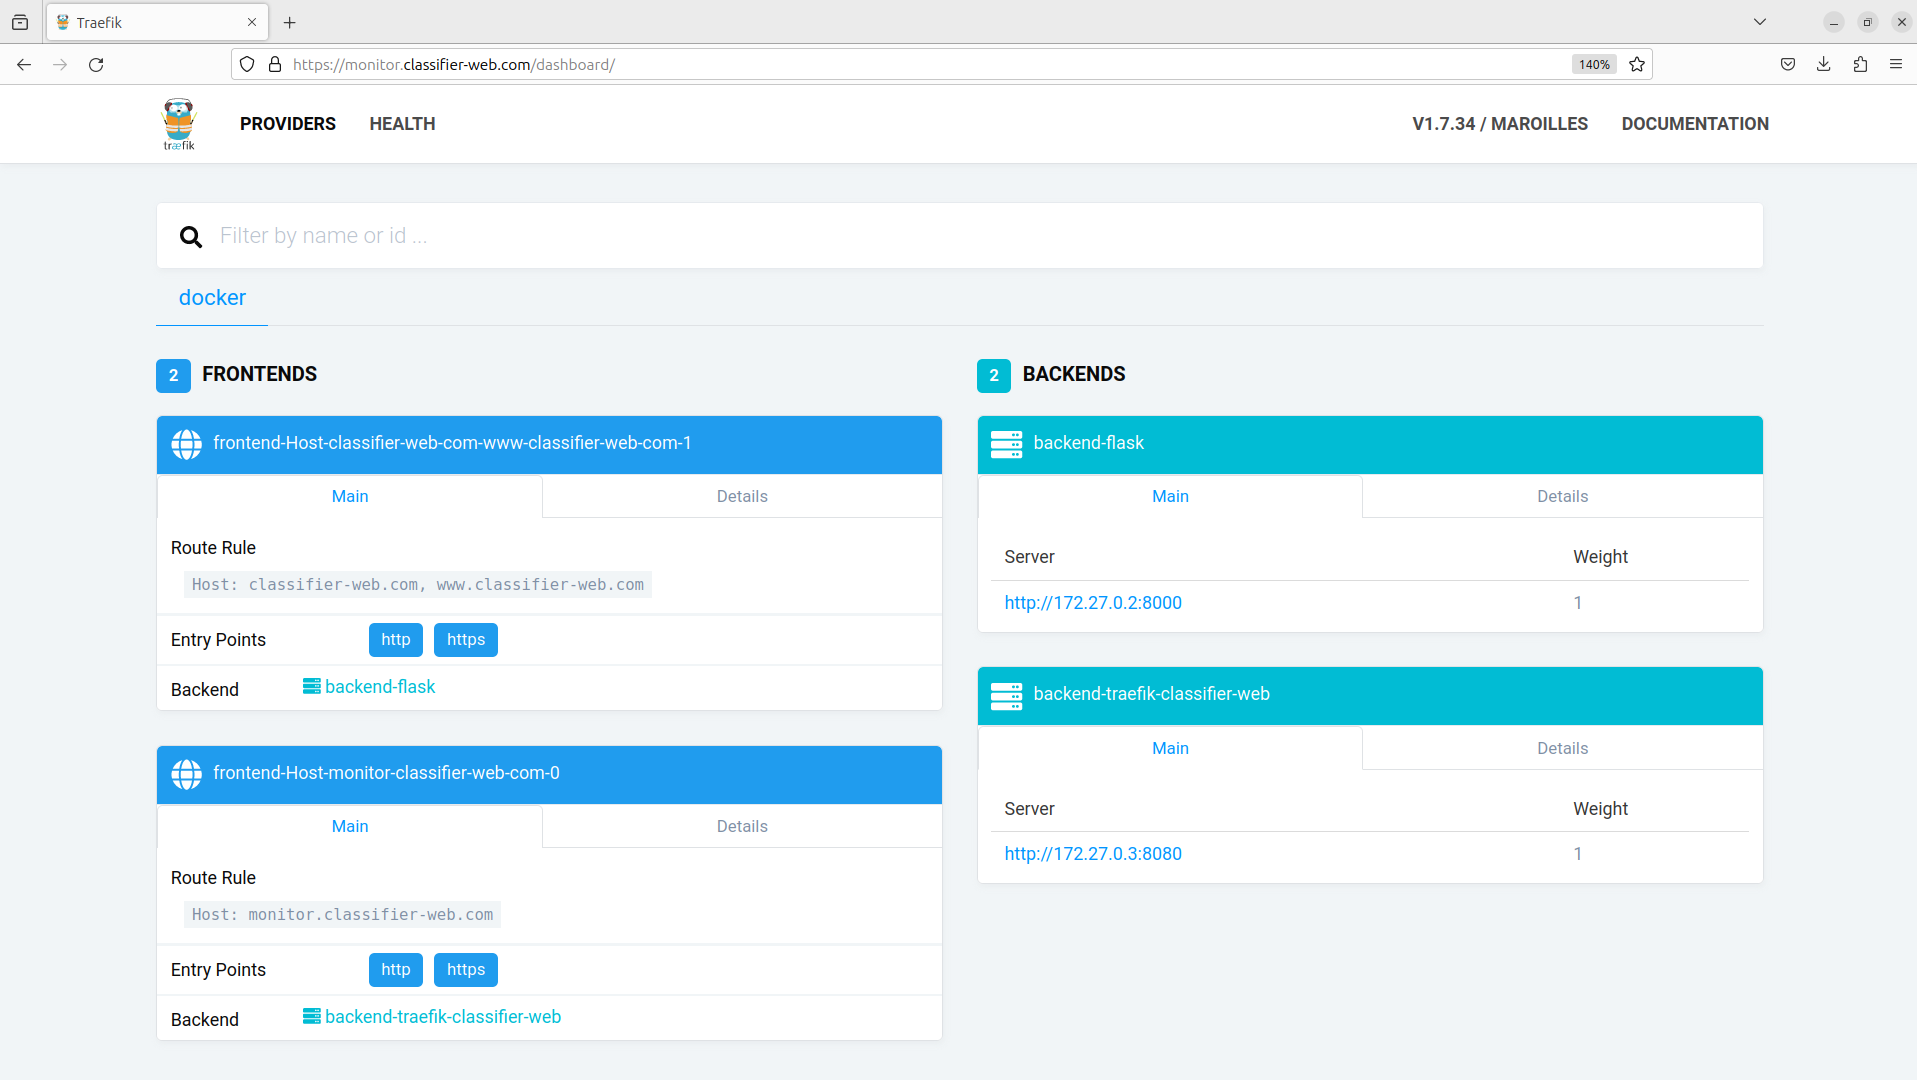
\includegraphics[width=0.8\textwidth]{cap3/images/monitor-dashboard.png}
    \caption{Panel de control de \textit{Traefik}, accesible a través de la dirección \url{https://monitor.classifier-web.com} con contraseña admin:admin}
    \label{fig:monitor-dashboard}
    
\end{figure}



\subsection{Docker}
Para facilitar el despliegue de la aplicación en cualquier entorno, se ha optado por utilizar contenedores Docker.
Esta tecnología permite encapsular una aplicación y sus dependencias en un contenedor, que puede ser ejecutado en cualquier entorno que tenga instalado Docker.
De este modo nos aseguramos que únicamente tenemos que preocuparnos de que el entorno tenga instalado Docker.

Esta tecnología ayuda a eliminar muchos problemas a la hora de desplegar servicios, pero incorpora otros de los que hay que ser conscientes.
En particular, Docker presenta un problema de seguridad, ya que los contenedores son ejecutados por defecto con privilegios de root.
Esto implicaría que si un atacante consigue acceder al contenedor, puede tener acceso a todo el sistema.

Este problema se ha solventado creando un usuario no privilegiado dentro del contenedor al construir la imagen de la aplicación, y ejecutando la aplicación con este usuario.
Sin embargo, las implicaciones de seguridad de Docker son un tema muy amplio y precisamente pueden llegar a ser determinantes para no utilizar esta tecnología en entornos de producción con requisitos de seguridad muy estrictos.
No es el caso de este trabajo, pero es un tema que hay que tener en cuenta y debería ser estudiado en profundidad antes de utilizar Docker en entornos de producción.

A pesar de ello, las ventajas que ofrece Docker son muy interesantes, y es una tecnología que ha ganando mucha popularidad en los últimos años.
Las principales ventajas que ofrece son las siguientes:

\begin{itemize}
    \item \textbf{Portabilidad}: Docker permite encapsular una aplicación y sus dependencias en un contenedor, que puede ser ejecutado en cualquier entorno que tenga instalado Docker.
    \item \textbf{Escalabilidad}: Docker permite crear múltiples contenedores de una misma aplicación, lo que permite escalar la aplicación de forma horizontal.
    \item \textbf{Aislamiento}: Docker permite aislar una aplicación y sus dependencias en un contenedor, lo que permite que la aplicación no se vea afectada por otras aplicaciones que se estén ejecutando en el mismo entorno.
\end{itemize}

Para este proyecto, hemos utilizado la imagen oficial de \textit{Traefik} y una imagen personalizada para la aplicación \textit{Flask}.
Para la construcción de la imagen de Flask, se ha utilizado una imagen base de \textit{Python} y se han instalado las dependencias necesarias para la aplicación.

\begin{lstlisting}[language=bash, caption={Dockerfile para la aplicación \textit{Flask}}, label={lst:dockerfile}]
FROM python:3.10.13

RUN apt update && apt upgrade -y
RUN apt install -y ffmpeg

# get curl for healthchecks
RUN apt install curl

# permissions and nonroot user for tightened security
RUN adduser nonroot
RUN mkdir /home/app/ && chown -R nonroot:nonroot /home/app
RUN mkdir -p /var/log/flask-app && touch /var/log/flask-app/flask-app.err.log && touch /var/log/flask-app/flask-app.out.log
RUN chown -R nonroot:nonroot /var/log/flask-app
WORKDIR /home/app
USER nonroot

# copy all the files to the container
COPY --chown=nonroot:nonroot . .

# venv
ENV VIRTUAL_ENV=/home/app/venv

# python setup
RUN python -m venv $VIRTUAL_ENV
ENV PATH="$VIRTUAL_ENV/bin:$PATH"
RUN export FLASK_APP=app.py


# upgrade pip
RUN pip install --upgrade pip

RUN pip install torch torchvision torchaudio --index-url https://download.pytorch.org/whl/cpu

# RUN pip install 'transformers[torch]'

RUN pip install -r requirements.txt


# define the port number the container should expose
EXPOSE 5000

CMD ["python", "app.py"]

\end{lstlisting}

\subsection{Docker Compose}
Docker Compose es una herramienta que permite definir y ejectutar aplicaciones Docker de forma sencilla.
Permite definir las imágenes de los contenedores, las redes, los volúmenes, etc., en un fichero YAML, y ejecutarlos con un único comando.

Es especialmente útil cuando se tienen varias aplicaciones que dependen unas de otras, ya que permite definir todas las aplicaciones en un único fichero.
En nuestro caso contamos solo con dos contenedores, pero crear un fichero Docker Compose nos permite definirlos de forma sencilla, construir las imágenes con las dependencias que nosotros definamos y levantar el despliegue con un único comando.

La sintaxis general de un fichero Docker Compose consiste en definir los servicios que se van a utilizar, las imágenes que se van a utilizar para cada servicio, los volúmenes que deben ser creados, las redes, variables de entorno, etc.

En este caso, algunos aspectos a destacar de la definición del fichero son los siguientes:

\begin{itemize}
    \item \textbf{Servicios}: Han sido definidos dos servicios, uno para la aplicación \textit{Flask} y otro para el servidor \textit{Traefik}.
    \item \textbf{Imagen}: Se ha utilizado la imagen oficial para el servidor \textit{Traefik}, y una imagen de \textit{Python} personalizada con las dependencias necesarias para la aplicación \textit{Flask}.
    \item \textbf{Volúmenes}: Para el servicio de \textit{Traefik} se han definido varios volúmenes para almacenar los certificados SSL y la configuración de \textit{Traefik}.
    \item \textbf{Redes}: No ha sido necesario definir ninguna red, ya que por defecto Docker Compose crea una red interna que es suficiente para que los contenedores se comuniquen entre sí.
    \item \textbf{Variables de entorno}: Han sido definidas varias variables principalmente para el servicio de \textit{Traefik}, de modo que pueda servir la aplicación \textit{Flask} con HTTPS.
\end{itemize}

El proyecto completo se puede encontrar en \url{https://github.com/antaramol/classifier-web}.

\begin{lstlisting}[language=bash, caption={Fichero Docker Compose.}, label={lst:docker-compose}]
version: '3'

services:
    flask:
    build: ./flask
    image: flask_app
    command: gunicorn -w 3 -t 60 -b 0.0.0.0:8000 app:app
    labels:
        - "traefik.enable=true"
        - "traefik.backend=flask"
        - "traefik.frontend.rule=Host: $DOMAIN_NAME, www.$DOMAIN_NAME"
        - "traefik.port=8000"

    traefik:
    image: traefik:1.7-alpine
    environment:
        - DOMAIN_NAME=$DOMAIN_NAME
    volumes:
        - /var/run/docker.sock:/var/run/docker.sock:ro
        - ./traefik/traefik.toml:/etc/traefik/traefik.toml:ro
        - ./traefik/acme:/etc/traefik/acme
        - ~/.htpasswd:/etc/htpasswd/.htpasswd
    labels:
        - "traefik.enable=true"
        - "traefik.frontend.rule=Host: monitor.$DOMAIN_NAME"
        - "traefik.port=8080"
    ports:
        - "80:80"
        - "443:443"
    

\end{lstlisting}


\begin{figure}[htpb]
    \centering
    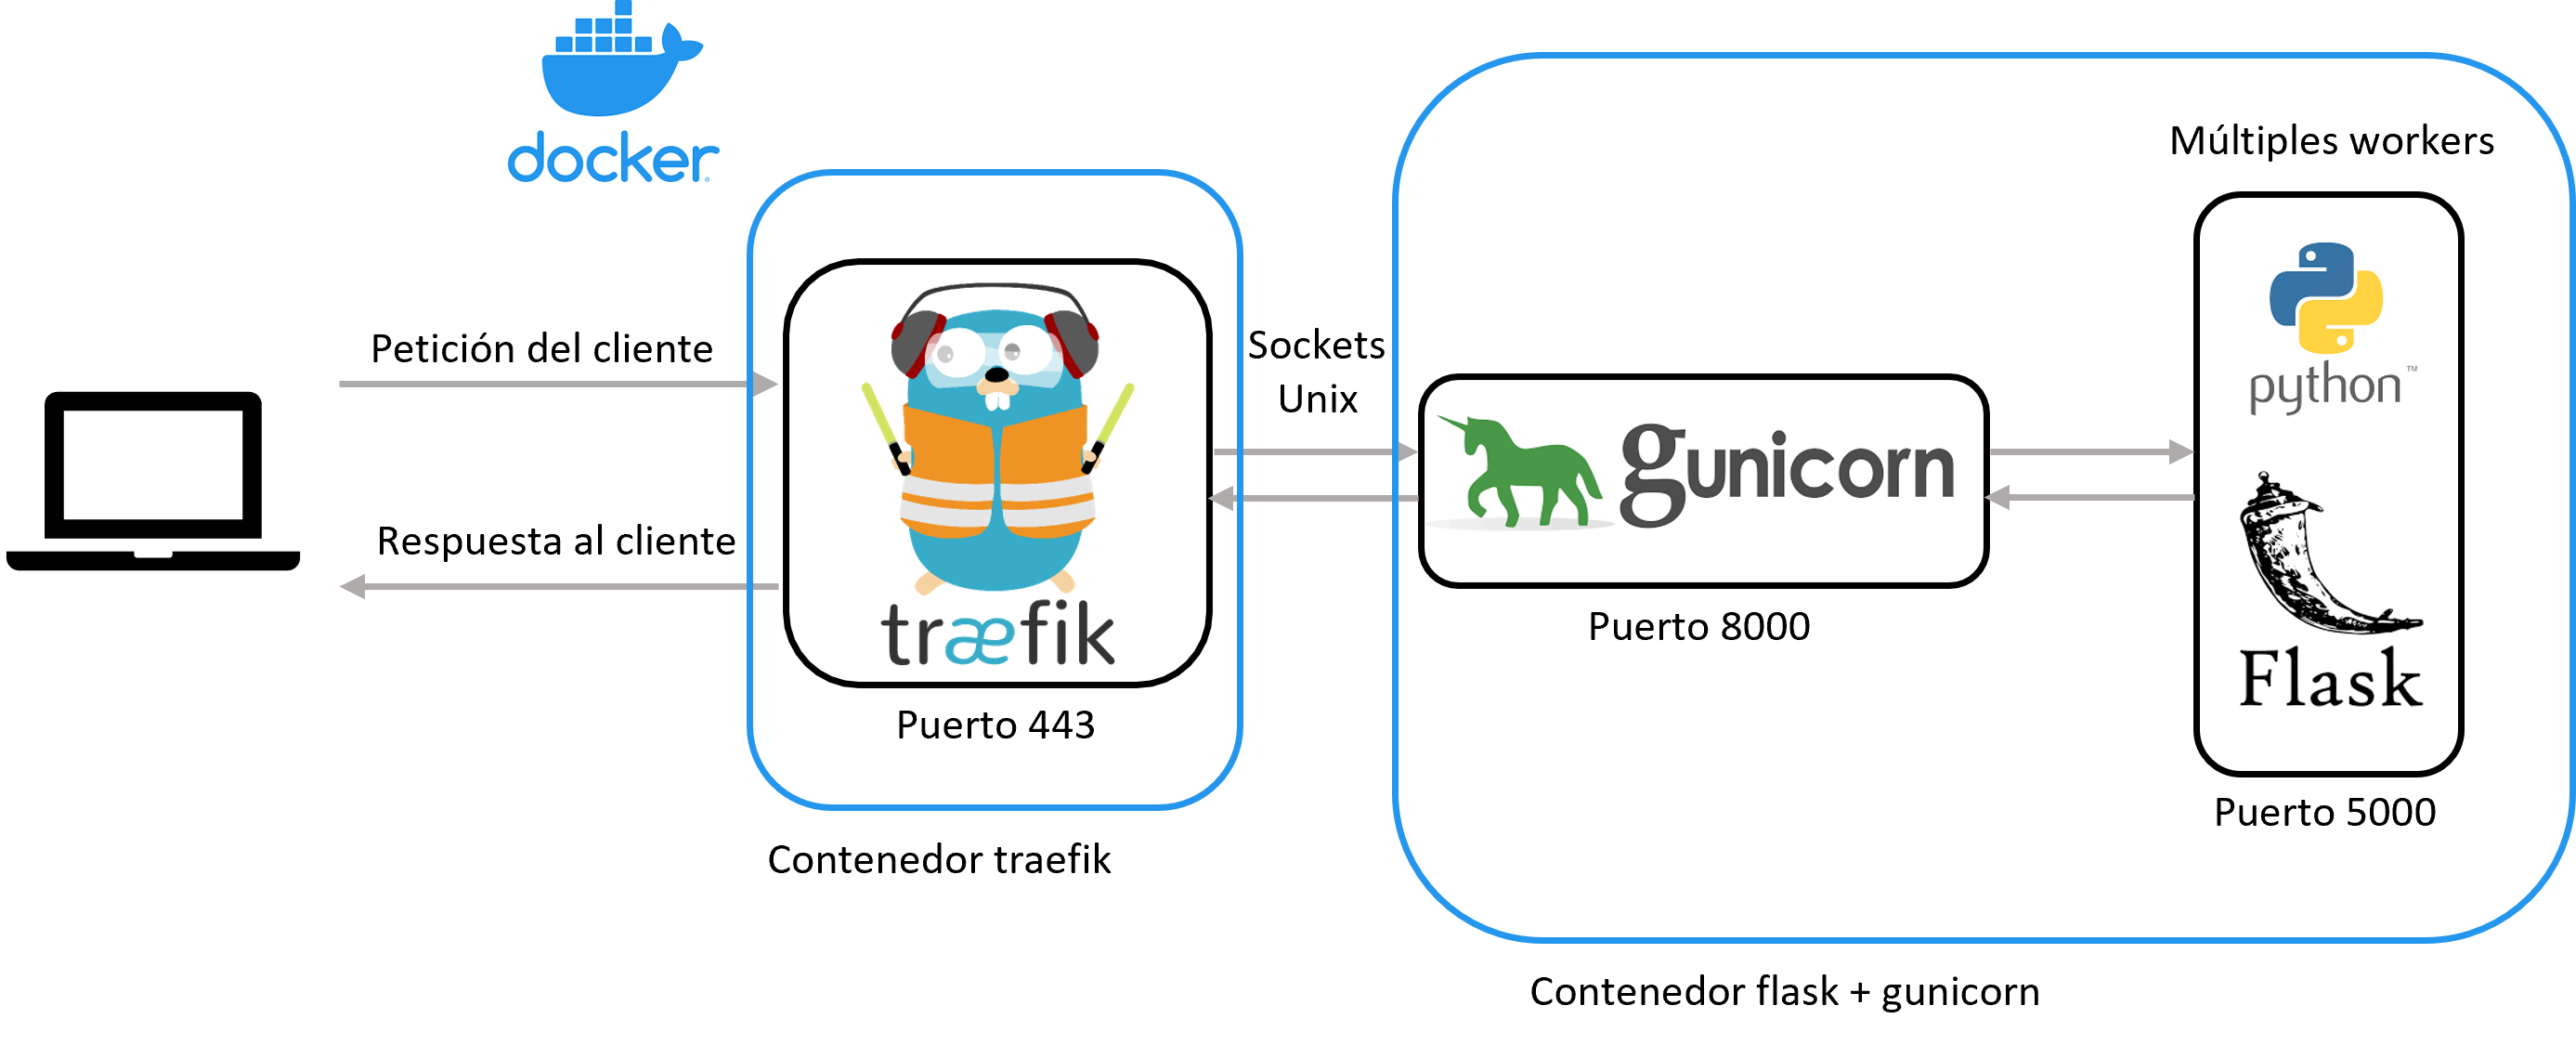
\includegraphics[width=0.8\textwidth]{cap3/images/arquitectura-docker.png}
    \caption{Esquema completo del sistema con Docker Compose}
    \label{fig:docker-compose}
\end{figure}

\section{Despliegue}
Una vez que la aplicación está lista para ser desplegada, es necesario elegir un entorno de producción.

Varias opciones han sido probadas para este trabajo, ya que no se tenía ninguna restricción en cuanto al entorno de producción.
Al no tener un servidor propio, se ha optado por utilizar servicios de terceros, que ofrecen servidores virtuales a un precio muy asequible.

De nuevo, igual que comentábamos en el apartado anterior, no es posible utilizar un ordenador personal para este servicio, ya que debería estar conectado todo el tiempo.
Además, existen cada vez más opciones de hosting y es muy interesante utilizarlas, ya que nos permiten centrarnos en el desarrollo de la aplicación y no en la gestión del servidor.

Esta es la principal ventaja, nos olvidamos de gestionar la infraestructura.
Además muchos servicios permiten gran facilidad para escalar horizontalmente, lo que nos permite aumentar la capacidad de la aplicación de forma sencilla.

Sin embargo, el principal problema es el coste, ya que estos servicios no son gratuitos.
Es un inconveniente que, sobre todo para iniciados en este mundo, puede ser determinante para no utilizar estos servicios.

Varias opciones han sido probadas para este trabajo, ya que cada una de ellas ofrece diferentes opciones y precios.

\subsection{Amazon Web Services}
Amazon Web Services (AWS) es una plataforma de servicios en la nube que ofrece servicios de computación, almacenamiento, bases de datos, etc.
Esta ha sido la primera opción probada debido a su gran popularidad y que se contaba con cierto conocimiento previo.

""" Insertar gráfico de popularidad"""

AWS ofrece una gran cantidad de servicios, y es una de las plataformas más completas que existen.
Este ha sido el principal problema, ya que está pensado para ser utilizado por empresas que necesitan una gran cantidad de servicios por su fácil integración entre ellos.
Como este trabajo solo necesita un servidor virtual, quizás AWS no sea la mejor opción.

En concreto, ha sido probado el servicio EC2, que ofrece servidores virtuales en la nube.
Cuenta con una capa gratuita, que permite utilizar un servidor virtual de forma gratuita durante un año, pero con ciertas limitaciones.

La capacidad de cómputo en la capa gratuita es muy limitada, pero es suficiente para probar la aplicación.
Sin embargo, el número de horas de uso es limitado, y una vez que se agotan, hay que pagar por cada hora de uso.
Esto hace que no sea una opción viable para este trabajo, ya que el coste sería muy elevado.
Este segmento está quizás pensado para pruebas puntuales de aplicaciones, pero no para desplegar aplicaciones en producción.

Sin embargo, sirvió para realizar diversas pruebas de funcionamiento, pruebas de rendimiento, etc., y para familiarizarse con este tipo de servicios.


\subsection{Google Cloud Platform}
El resultado es similar al de AWS, ya que Google Cloud Platform (GCP) está enfocado igualmente a grandes proyectos.

Además, la documentación de estos servicios es tan extensa que puede llegar a ser abrumadora para un desarrollador que no esté familiarizado con este tipo de servicios.
Una mejor opción para este trabajo es utilizar servicios más sencillos, que estén pensados para pequeños proyectos y que sean más fáciles de utilizar, suavizando así la curva de aprendizaje.

La atracción hacia Google Cloud Platform es que ofrece una gran cantidad de crédito gratuito para utilizar sus servicios, lo que permite utilizarlos de forma gratuita durante un tiempo.
El resultado es muy similar a AWS, esta vez se ha utilizado el servicio Compute Engine, que ofrece servidores virtuales en la nube.


\subsection{VPS}
Una opción más sencilla y económica es utilizar un VPS (Virtual Private Server), que es un servidor virtual que se encuentra alojado en un servidor físico.
Este tipo de servidores cuentan con una ventaja con respecto a los anteriores, y es que el precio es fijo, y no depende del uso que se haga del servidor.

En concreto, se ha utilizado el servicio de VPS de Contabo, recomendado por un compañero de la universidad.
Este servicio ofrece servidores virtuales a un precio muy asequible, y con una gran cantidad de recursos.

Es muy sencillo desplegar una instancia de un servidor virtual, a la que podemos conectarnoso mediante SSH.
Si a esto le sumamaos la facilidad que nos ofrece Docker Compose para desplegar la aplicación, junto con herramientas de edición como VSCode que nos permiten conectarnos y 
editar los ficheros de la aplicación de forma remota, el resultado es muy satisfactorio.

\begin{figure}[htpb]
    \centering
    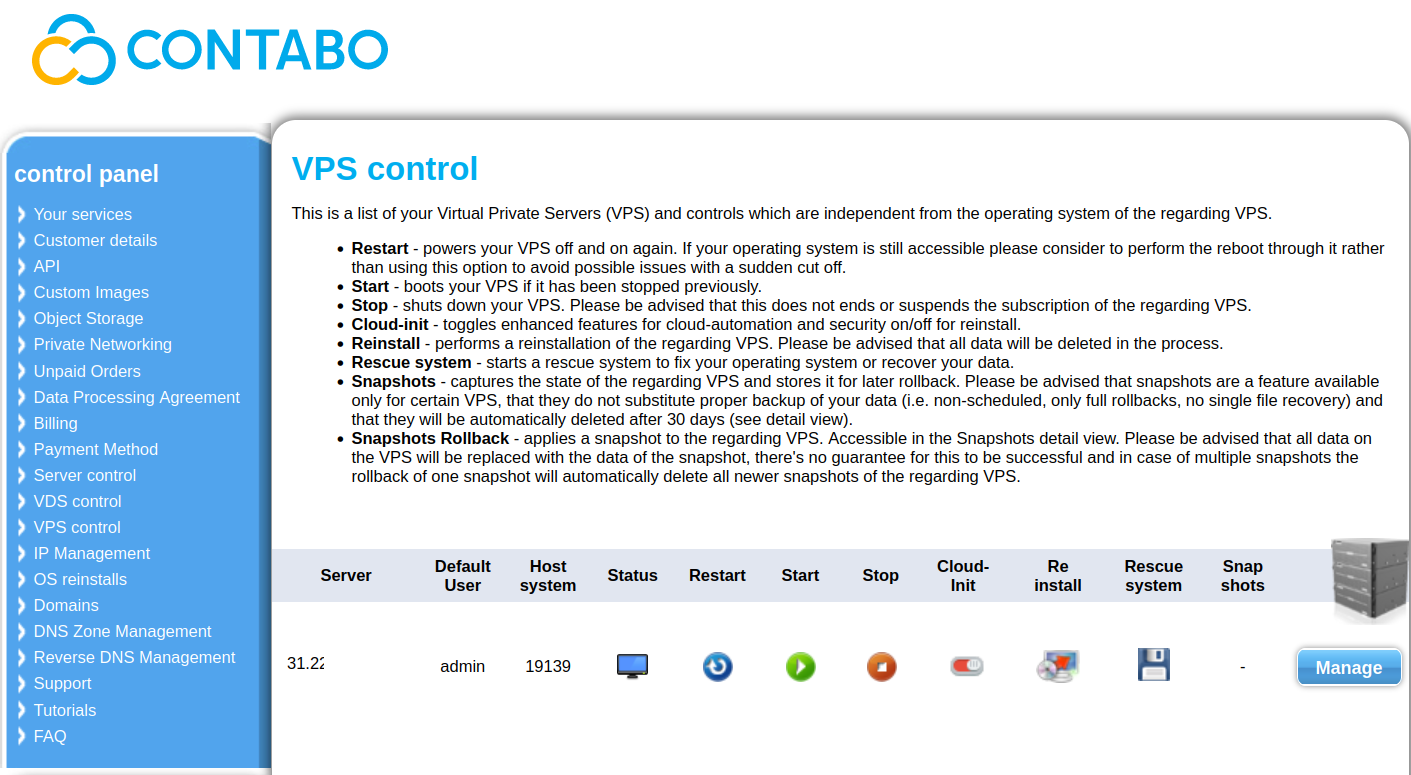
\includegraphics[width=0.8\textwidth]{cap3/images/contabo-instance.png}
    \caption{Instancias activas en Contabo}
    \label{fig:contabo}
\end{figure}

Contabo además nos ofrece muchas opciones que nos ayudan a perfilar el resultado final.
En nuestro caso, se ha utilizado el área de manejo de DNS para configurar el dominio de la aplicación, de modo que podemos otorgarle un nombre más amigable a la aplicación.
Contabo permite crear registros DNS de forma sencilla, y además ofrece un servicio de DNS dinámico, que permite asignar un nombre de dominio a una IP dinámica, que es la que nos ofrece el servidor virtual.

\begin{figure}[htpb]
    \centering
    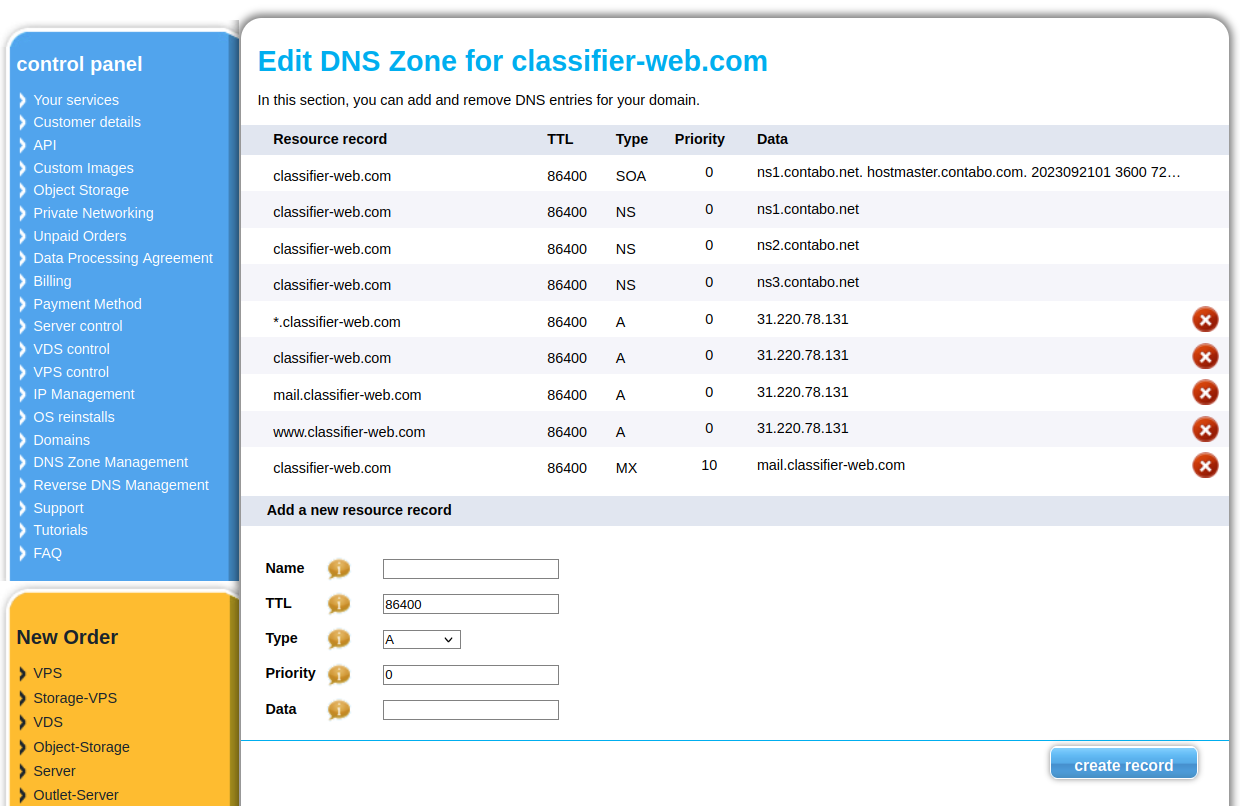
\includegraphics[width=0.8\textwidth]{cap3/images/contabo-dns.png}
    \caption{Configuración de DNS en Contabo}
    \label{fig:contabo-dns}
\end{figure}

Para esta aplicación, se ha elegido un servidor de 4 núcleos, 8 GB de RAM y 50 GB de almacenamiento.
Si en un futuro se necesitara más capacidad, se podría escalar horizontalmente, creando más instancias de la aplicación y balanceando la carga entre ellas.
Para esta implementación, quizás sería más conveniente estudiar en profundidad los servicios de AWS o GCP, ya que ofrecen más facilidades para escalar horizontalmente, pero para el propósito de este trabajo, es más que suficiente.





\endinput